\chapter{Implementierung}
In diesem Kapitel wird auf Implementierungsdetails des Entwurfs eingegangen. Hierbei ist zu beachten, dass aus Platzgründen der vorliegende Code eventuell in gekürzter oder geänderter Form dargestellt wird und unvollständig ist. Dennoch verdeutlichen die Codebeispiele die wesentlichsten Details der Implementierung und sind gemäß des Entwurfs umgesetzt.

\section{Verarbeitungskette}
Die Verarbeitungskette ist ein Teil des \texttt{AudioHandlers} und einer der wichtigen Komponenten des Frameworks. Sie ist die Schnittstelle mit der anderen Klassen an der Audioverarbeitung teilnehmen können. Im folgenden Kapitel wird erörtert wie diese implementiert wurde.

\subsection{Interface für Audioverarbeitungsklassen}
Alle Audioverarbeitungsklassen müssen die abstrakte Klasse \texttt{AudioProcessor} implementieren, siehe Listening \ref{Code:AudioProcessor}.

\begin{lstlisting}[caption={Interface des AudioProcessors},label={Code:AudioProcessor}]
class AudioProcessor {
public:
	AudioProcessor(const std::string name);
	virtual unsigned int processInputData(void *inputBuffer, int inputBufferByteSize) = 0;
	virtual unsigned int processOutputData(void *outputBuffer,  int outputBufferByteSize) = 0;
}
\end{lstlisting}
Der Konstruktor in Zeile 4 erwartet als Parameter den Namen des Audioprozessors, damit dieser später eindeutig identifiziert werden kann. Die beiden Verarbeitungsmethoden in Zeile 5 und 6 sind virtuell, daher müssen alle Unterklassen diese implementieren. Diese Methoden stellen die Schnittstelle zur Audioverarbeitung dar und haben als Parameter jeweils den Buffer sowie die Buffergröße.

\subsection{An- und Abmeldeprozess im AudioHandler}
Listening \ref{Code:AudioHandlerAdd} zeigt die Schnittstelle zum An- und Abmelden von Audioprozessoren im \texttt{AudioHandlers} an. Die Methode \texttt{addProcessor()} fügt einen Audioprozessor in die Audioverarbeitungsliste ein, falls er noch nicht vorhanden ist, und \texttt{removeProcessor()} ist die entsprechende Löschmethode. Als Liste wird hier der Standardcontainer \texttt{std::vector} benutzt. Bei diesem werden neue Elemente am Ende der Liste eingefügt.

\begin{lstlisting}[caption={An- und Abmeldeprozess von Audioprozessoren im AudioHandler},label={Code:AudioHandlerAdd}]
bool AudioHandler::addProcessor(AudioProcessor *audioProcessor)
{
	if (hasAudioProcessor(audioProcessor) == false) {
		audioProcessors.push_back(std::unique_ptr<AudioProcessor>(audioProcessor));
		return true;
	}
	return false;
}

bool AudioHandler::removeAudioProcessor(AudioProcessor *audioProcessor) {
	for (size_t i = 0; i < audioProcessors.size(); i++)
	{
		if ((audioProcessors.at(i))->getName() == audioProcessor->getName()) {
			audioProcessors.erase(audioProcessors.begin() + i);
			return true;
		}	
	}
	return false;
}
\end{lstlisting}

\subsection{Verarbeitungsprozess}
Listening \ref{Code:AudioHandlerProcess} zeigt den Verarbeitungsprozess. Die Methode \texttt{processAudioInput()} wird vom AudioHandler aufgerufen, falls Daten vom Mikrofon zur Verarbeitung anliegen. Dort wird von jedem angemeldeten Audioprozessor die entsprechende \texttt{processInputData()} -Methode aufgerufen. Als Parameter werden die Daten des Mikrofons und deren Datengröße übergeben. Die Verarbeitungsreihenfolge entspricht der Anmeldereihenfolge. Die Verarbeitung im Buffer erfolgt in-place, daher auf den übergebenen Buffer. Falls ein Audioprozessor zu Beginn die Daten manipuliert, so sind diese Daten für alle nachfolgenden Prozessoren ebenfalls geändert. Im Umkehrschluss heißt dies, um wieder an die Ursprungsdaten zu gelangen, müssen die ausgeführten Änderungen in umgekehrte Reihenfolge rückgängig gemacht zu werden. \texttt{processAudioOutput()} wird aufgerufen, wenn die Soundkarte bereit ist Audiodaten abzuspielen. Hierzu werden von allen Audioprozessoren die \texttt{processOutputData()} - Methoden aufgerufen, jedoch mit umgekehrter Aufrufreihenfolge, siehe Zeile 13. Dadurch wird der Ursprungszustand der Audiodaten hergestellt und sind abspielbar.

\begin{lstlisting}[caption={Verarbeitungsprozess des AudioHandlers},label={Code:AudioHandlerProcess}]
void AudioHandler::processAudioInput(void *inputBuffer,  int inputBufferByteSize)
{
	unsigned int bufferSize = inputBufferByteSize;
	for (unsigned int i = 0; i < audioProcessors.size(); i++)
	{
		bufferSize = audioProcessors.at(i)->processInputData(inputBuffer, bufferSize);
	}
}

void AudioHandler::processAudioOutput(void *outputBuffer, int outputBufferByteSize)
{
	unsigned int bufferSize = outputBufferByteSize;
	for (unsigned int i = audioProcessors.size(); i > 0; i--)
	{
		bufferSize = audioProcessors.at(i-1)->processOutputData(outputBuffer, bufferSize);
	}
}
}\end{lstlisting}

\section{Factory-Klassen}
Die beiden Factory-Klassen \texttt{AudioHandlerFactory} und \texttt{AudioProcessorFactory} sind vom Aufbau identisch, deshalb wird im folgenden nur die \texttt{AudioHandlerFactory} erklärt. \texttt{AudioProcessorFactory} verhält sich analog dazu. Die Factory-Klassen haben die Aufgabe die Instantiierung in Methoden auszulagern, damit das Programmieren auf Schnittstellen gewährleistet wird. Methoden die Instantiierung übernehmen werden auch Fabrikmethoden genannt \cite{Goll2013}[S.243]. Listening \ref{Code:AudioHandlerFactory} zeigt die Fabrikmethode der \texttt{AudioHandlerFactory}. Als Parameter wird der Name der zu erzeugende Klasse entgegen genommen. Der Rückgabewert der Funktion entspricht den abstrakten und gemeinsamen Basistypen.

\begin{lstlisting}[caption={Fabrikmethode der AudioHandlerFactory},label={Code:AudioHandlerFactory}]
std::unique_ptr<AudioHandler> AudioHandlerFactory::getAudioHandler(std::string name) {
	if (name == RTAUDIO_WRAPPER)
	{
		std::unique_ptr<RtAudioWrapper> rtaudiowrapper(new RtAudioWrapper);
		return std::move(rtaudiowrapper);
	}
	throw std::invalid_argument("No AudioHandler for this name!");
}
\end{lstlisting}

\section{RTPListener}
\texttt{RTPListener} ermöglicht das asynchrone Empfangen von Paketen durch das Erstellen eines eignen Threads. Die wichtigsten Methoden der Klasse sind im Listening \ref{Code:RTPListener} dargestellt. Die \texttt{startUp()}-Methode startet den Thread und \texttt{shutdown()} beendet ihn wieder. Sobald der Thread startet wird \texttt{runThread()} aufgerufen. Tatsächlich ist diese Methode komplexer, wurde jedoch für das Beispiel auf das wesentliche gekürzt. In der Schleife wird die blockierende \texttt{receiveData()}-Funktion aufgerufen. Übertragene Packete werden im Jitter-Buffer zwischengespeichert, siehe Zeile 14. Die empfangenen Pakete können anschließend aus dem Jitter-Buffer von anderen Threads ausgelesen werden. Der \texttt{RTPListener} wartet anschließend wieder auf neue ankommende Pakete.

\begin{lstlisting}[caption={Die wichtigsten Methoden des RTPListeners},label={Code:RTPListener}]
void RTPListener::startUp()
{
    threadRunning = true;
    receiveThread = std::thread(&RTPListener::runThread, this);
}

void RTPListener::shutdown(){
	threadRunning = false;
}

void RTPListener::runThread() {
	while(threadRunning) {
		int receivedSize = this->wrapper->receiveData(rtpHandler.getWorkBuffer(), rtpHandler.getMaximumPackageSize());
		auto result = buffer->addPackage(rtpHandler, receivedSize - RTP_HEADER_MIN_SIZE);
	}
}
\end{lstlisting}

\section{RtAudio}

Der RtAudioWrapper bietet drei Modi zur Audiokommunikation, diese sind RecordingMode, PlaybackMode und DuplexMode. Bei den ersten beiden Modi wird entweder nur der input oder der output Stream übergeben um nur Sound aufzunehmen oder abzuspielen. Dagegen benutzt der letzte Modus DuplexMode den input und output Stream um ein simultanes aufnehmen und abspielen von Audio Daten zu ermöglichen.

Die RtAudio-API wird mittels eines Objekts, dessen Namen auf rtaudio definiert wurde gesteuert.

\begin{lstlisting}[caption={RtAudio Objekt und StreamParameter},label={Code:RtAudio}]
RtAudio rtaudio;
RtAudio::StreamParameters input, output;
\end{lstlisting}

Zu beginn wird per Flag(flagPrepare) geprüft ob die prepare()-Methode von RtAudioWrapper ausgeführt wurde - welche überprüft ob die Output und Input Stream Parameter konfiguriert wurden - und alle AudioProzessoren mittels der prepare()-Methode des AudioHandler ihre Unterstützten Parameter gemeldet haben und sich auf einen gleichen Parametersatz einigen konnten. Wenn dies nicht der Fall ist wird ein Fehler ausgegeben mit dem Hinweis das die AudioProzessoren zuerst konfiguriert werden müssen bevor der RtAudio Stream gestartet werden kann.

Dem rtaudio Objekt werden per openStream()-Methode die benötigten Parameter mitgeteilt, welche folgenden Inhalt haben:

\begin{description}
\item[output] Der Output Stream Parameter welcher die deviceID also die ID des Hardware Geräts welches die Audio Signale ausgeben soll und die Anzahl der zu benutzenden Channels enthält. Diese wurden entweder per setDefaultAudioConfig()-Methode des RtAudioWrapper oder per FileConfiguration, InteractiveConfiguration oder ParameterConfiguration festgelegt.
\item [input] Der Input Parameter welcher die deviceID des Audio Geräts - welches die Audio Signale aufnimmt - und die Anzahl der aufzunehmenden Channels enthält. Dieser wurde ebenfalls vorher mittels einer der verschiedenen Konfigurations-Modi konfiguriert.
\item [audioConfiguration.audioFormatFlag] : Das Audio Format Flag welches das Audio Format definiert welches durch den AudioHandler durch abfragen der AudioProzessoren ausgehandelt wurde.
\item [audioConfiguration.sampleRate] Die Sample Rate welche vom AudioHandler durch abfragen der AudioProzessoren ausgehandelt wurde.
\item [audioConfiguration.framesPerPackage] Die Anzahl der Frames per Package also die Größe des Audio Buffers. Diese Größe wurde auch vom AudioHandler durch abfragen der AudioProzessoren ausgehandelt
\item [RtAudioWrapper::callbackHelper] Die Callback Methode welche von der RtAudio-API aufgerufen wird wenn Audio Daten vorhanden sind.
\item [this] Eine Referenz auf das eigene Callback Objekt. Um innerhalb der Callback Methode auf benötigte Informationen zuzugreifen.
\end{description}

Anschließend wird die RtAudio-API mittels startStream() gestartet.

\begin{lstlisting}[caption={Start des Duplex Mode im RtAudioWrapper},label={Code:RtAudio}]
void RtAudioWrapper::startDuplexMode()
{
    if (this->flagPrepared)
    {
        this->rtaudio.openStream(&output, &input, audioConfiguration.audioFormatFlag, audioConfiguration.sampleRate, &audioConfiguration.framesPerPackage, &RtAudioWrapper::callbackHelper, this);
        this->rtaudio.startStream();
    }
    else
        std::cout << "Did you forget to call AudioHandler::prepare()?" << std::endl;
}
\end{lstlisting}

Der callbackHelper erstellt daraufhin ein rtAudioWrapper Objekt und ruft dessen callback Methode auf. \textcolor{red}{TODO: Begründung wieso zweistufiger Callback}

\begin{lstlisting}[caption={callbackHelper Methode im RtAudioWrapper},label={Code:RtAudio}]
auto RtAudioWrapper::callbackHelper(void *outputBuffer, void *inputBuffer, unsigned int nBufferFrames, double streamTime, RtAudioStreamStatus status, void *rtAudioWrapperObject) -> int
{
    RtAudioWrapper *rtAudioWrapper = static_cast <RtAudioWrapper*> (rtAudioWrapperObject);
    return rtAudioWrapper->callback(outputBuffer, inputBuffer, nBufferFrames, streamTime, status, nullptr);
}
\end{lstlisting}

Welche die processAudioInput und processAudioOutput Methode aufruft und somit die einzelnen Prozessoren durchläuft.

\begin{lstlisting}[caption={callback Methode im RtAudioWrapper},label={Code:RtAudio}]
auto RtAudioWrapper::callback(void *outputBuffer, void *inputBuffer, unsigned int nBufferFrames, double streamTime, RtAudioStreamStatus status, void *rtAudioWrapperObject) -> int
{
	(...)
	this->processAudioInput(inputBuffer, inputBufferByteSize, streamData);
	(...)
	this->processAudioOutput(outputBuffer, outputBufferByteSize, streamData);
	
	return 0;
}
\end{lstlisting}

\section{Opus}

Der Opus Codec welcher zum encoden und decoden der Audio Daten benutzt wird wurde als Prozessor in OHMComm eingebunden.

Der Konstruktor des Opus Prozessor erstellt bei der Instanziierung jeweils ein Encoder und Decoder Objekt. Außerdem wird ihm ein Name gegeben und der Opus Application Type\textcolor{red}{TODO: ref OpusApplication Type im Entwurf} wird gewählt.

\begin{lstlisting}[caption={Instanziierung des Opus Prozessors},label={Code:Opus}]
ProcessorOpus::ProcessorOpus(const std::string name, int opusApplication) : 
    AudioProcessor(name), OpusEncoderObject(nullptr), OpusDecoderObject(nullptr)
{
    this->OpusApplication = opusApplication;
}
\end{lstlisting}

Das Encodieren der Audio Daten geschieht in der processInputData()-Methode des Opus Prozessors. Zu Beginn wird die Variable lengthEncodedPacketInBytes deklariert in welcher die Größe der Audio Daten nach ihrer Encodierung gespeichert wird. Anschließend wir geprüft ob Daten im Signed Inter 16 Format oder im Float 32 Format vorliegen.
Abhängig davon wir die opus\_encode()-Methode aufgerufen welche folgende Parameter benötigt:

\begin{description}
\item[OpusEncoderObject] Das bei der Instanziierung erzeugte und in der configure()-Methode konfigurierte Opus Encoder Objekt.
\item[(opus\_int16 *)inputBuffer] Der ins opus\_int16 oder Float 32 Format gecastete InputBuffer Pointer welcher die Input Audio Daten der Soundkarte enthält.
\item[userData->nBufferFrames] Die Anzahl der Samples(per Channel) welche sich im InputBuffer befinden.
\item[(unsigned char *)inputBuffer] Char-Pointer der Anzeigt wohin die Encodierten Audio Daten geschrieben werden sollen. Da wir auf dem inputBuffer Arbeiten und keinen extra Speicherplatz für Encodierte Daten haben, ist dies der selbe Speicherbereich aus dem wir die Daten gelesen haben.
\item[userData->maxBufferSize] Maximal Größe des Speicherbereichs wohin die Encodierten Daten geschrieben werden.
\end{description}

Als Rückgabewert geben wir die neue Größe des inputBuffers weiter. 


\begin{lstlisting}[caption={Encodieren von Audio Daten mittels Opus},label={Code:Opus}]
unsigned int ProcessorOpus::processInputData(void *inputBuffer, const unsigned int inputBufferByteSize, StreamData *userData)
{
    unsigned int lengthEncodedPacketInBytes = 0;
    if (rtaudioFormat == AudioConfiguration::AUDIO_FORMAT_SINT16)
    {
        lengthEncodedPacketInBytes = opus_encode(OpusEncoderObject, (opus_int16 *)inputBuffer, userData->nBufferFrames, (unsigned char *)inputBuffer, userData->maxBufferSize);
        return lengthEncodedPacketInBytes;
    }
    else if (rtaudioFormat == AudioConfiguration::AUDIO_FORMAT_FLOAT32)
    {
        lengthEncodedPacketInBytes = opus_encode_float(OpusEncoderObject, (const float *)inputBuffer, userData->nBufferFrames, (unsigned char *)inputBuffer, userData->maxBufferSize);
        return lengthEncodedPacketInBytes;
    }
    else
    {
        std::cerr << "[Opus-processInputData-Error]No matching encoder found, AudioFormat possibly not supported" << std::endl;
        return 0;
    }
}
\end{lstlisting}

Das Decodieren geschieht auf ähnliche weise wie das Encodieren der Audio Daten.
Zuerst wird eine Variable angelegt in welcher wir die Anzahl der Decodierten Samples speichern (numberOfDecodedSamples) welche wir von der opus\_decode()-Methode als Rückgabewert bekommen. Es wird wieder geprüft ob die Daten im Signed Integer 16 Format oder im Float 32 Format decodiert werden sollen. Anschließend wird die opus\_decode()-Methode mit folgenden Parametern aufgerufen :

\begin{description}
\item[OpusDecoderObject] Das bei der Instanziierung erzeugte und in der configure()-Methode konfigurierte Opus Decoder Objekt.
\item[(unsigned char *)outputBuffer] Char Pointer auf die Encodierten Audio Daten
\item[outputBufferByteSize] Größe des OutputBuffers
\item[(opus\_int16 *)outputBuffer] Pointer wohin die Decodierten Audio Daten geschrieben werden sollen entweder im Signed Integer 16 oder Float 32 Format.
\item[userData->maxBufferSize] Maximal Größe des Speicherbereichs welcher die Decodierten Daten aufnimmt.
\item[0] Möglicher Platz für ein Flag welches Anzeigt ob in-band forward error correction data vorhanden ist, was nicht der Fall ist.
\end{description}

Da wir als Rückgabewert von opus\_decode() die Anzahl der Decodierten Samples bekommen, die Prozessoren aber als Rückgabewert die Größe des OutputBuffers zurückgeben sollen muss diese noch Mittels der Anzahl der Decodierten Samples mal der Größe des gewünschten Formates mal der Anzahl der Channels (numberOfDecodedSamples * sizeof(opus\_int16) * outputDeviceChannels) berechnet werden.

\begin{lstlisting}[caption={Decodieren von Audio Daten mittels Opus},label={Code:Opus}]
unsigned int ProcessorOpus::processOutputData(void *outputBuffer, const unsigned int outputBufferByteSize, StreamData *userData)
{
    unsigned int numberOfDecodedSamples = 0;
    if (rtaudioFormat == AudioConfiguration::AUDIO_FORMAT_SINT16)
    {
        numberOfDecodedSamples = opus_decode(OpusDecoderObject, (unsigned char *)outputBuffer, outputBufferByteSize, (opus_int16 *)outputBuffer, userData->maxBufferSize, 0);
        userData->nBufferFrames = numberOfDecodedSamples;
        const unsigned int outputBufferInBytes = (numberOfDecodedSamples * sizeof(opus_int16) * outputDeviceChannels);
        return outputBufferInBytes;
    }
    else if (rtaudioFormat == AudioConfiguration::AUDIO_FORMAT_FLOAT32)
    {
        numberOfDecodedSamples = opus_decode_float(OpusDecoderObject, (const unsigned char *)outputBuffer, outputBufferByteSize, (float *)outputBuffer, userData->maxBufferSize, 0);
        userData->nBufferFrames = numberOfDecodedSamples;
        const unsigned int outputBufferInBytes = (numberOfDecodedSamples * sizeof(float) * outputDeviceChannels);
        return outputBufferInBytes;
    }
    else
    {
        std::cerr << "[Opus-processOutputData-Error]No matching decoder found, AudioFormat possibly not supported" << std::endl;
        return 0;
    }
}
\end{lstlisting}

\FloatBarrier
\section{Passive Konfiguration}
\label{passiveConfiguration}
Die passive Konfiguration aus Abschnitt \ref{configurationUsages} wird mithilfe von \textbf{Application-defined} RTCP-Paketen aus Abschnitt \ref{rtcp} umgesetzt. Hierfür wird für die Konfiguration einer Sitzung der Klient \textbf{A} mit der Option \enquote{Konfigurations-Anfrage aktivieren} (oder dem Parameter \texttt{--wait-for-passive}) gestartet, um eine Anfrage einer passiven Konfiguration zu ermöglichen. Klient \textbf{B} wird mit dem Parameter \texttt{--passive} ausgeführt. Klient \textbf{A} konfiguriert das OHMComm-Framework, startet jedoch noch keine Kommunikation, sondern nur den RTCP-Thread und wartet dort auf eine Anfrage für eine passive Konfiguration. Klient \textbf{B} sendet eine RTCP Application-defined Nachricht an \textbf{A}, die die Anfrage einer passiven Konfiguration darstellt. Daraufhin antwortet \textbf{A} mit einem weiteren RTCP-Paket, das die Werte der passiven Konfiguration (Abtastrate, Audioformat, Audiocodecs, Anzahl der Kanäle sowie die Puffergröße) beinhaltet. Dieses Paket wird von \textbf{B} empfangen und die Konfiguration ausgelesen. Daraufhin können beide Seiten das Übertragen von Audiodaten beginnen. Durch die Übertragung aller relevanten Informationen (Einstellungen der Audiobibliothek sowie die verwendeten Audiocodecs) wird garantiert, dass die gesendeten Daten von der anderen Instanz auch verstanden und verwendet werden können. Um die passive Konfiguration zu starten, wird für den Klienten \textbf{B} nur die IP-Adresse und der Port des Klienten \textbf{A} benötigt, wohingegen \textbf{A} komplett wie bereits beschrieben konfiguriert werden kann. Der Ablauf einer passiven Konfiguration ist schematisch in Listing \ref{lst:passiveConfiguration} dargestellt:
\newline
\begin{figure}[htp]
\centering
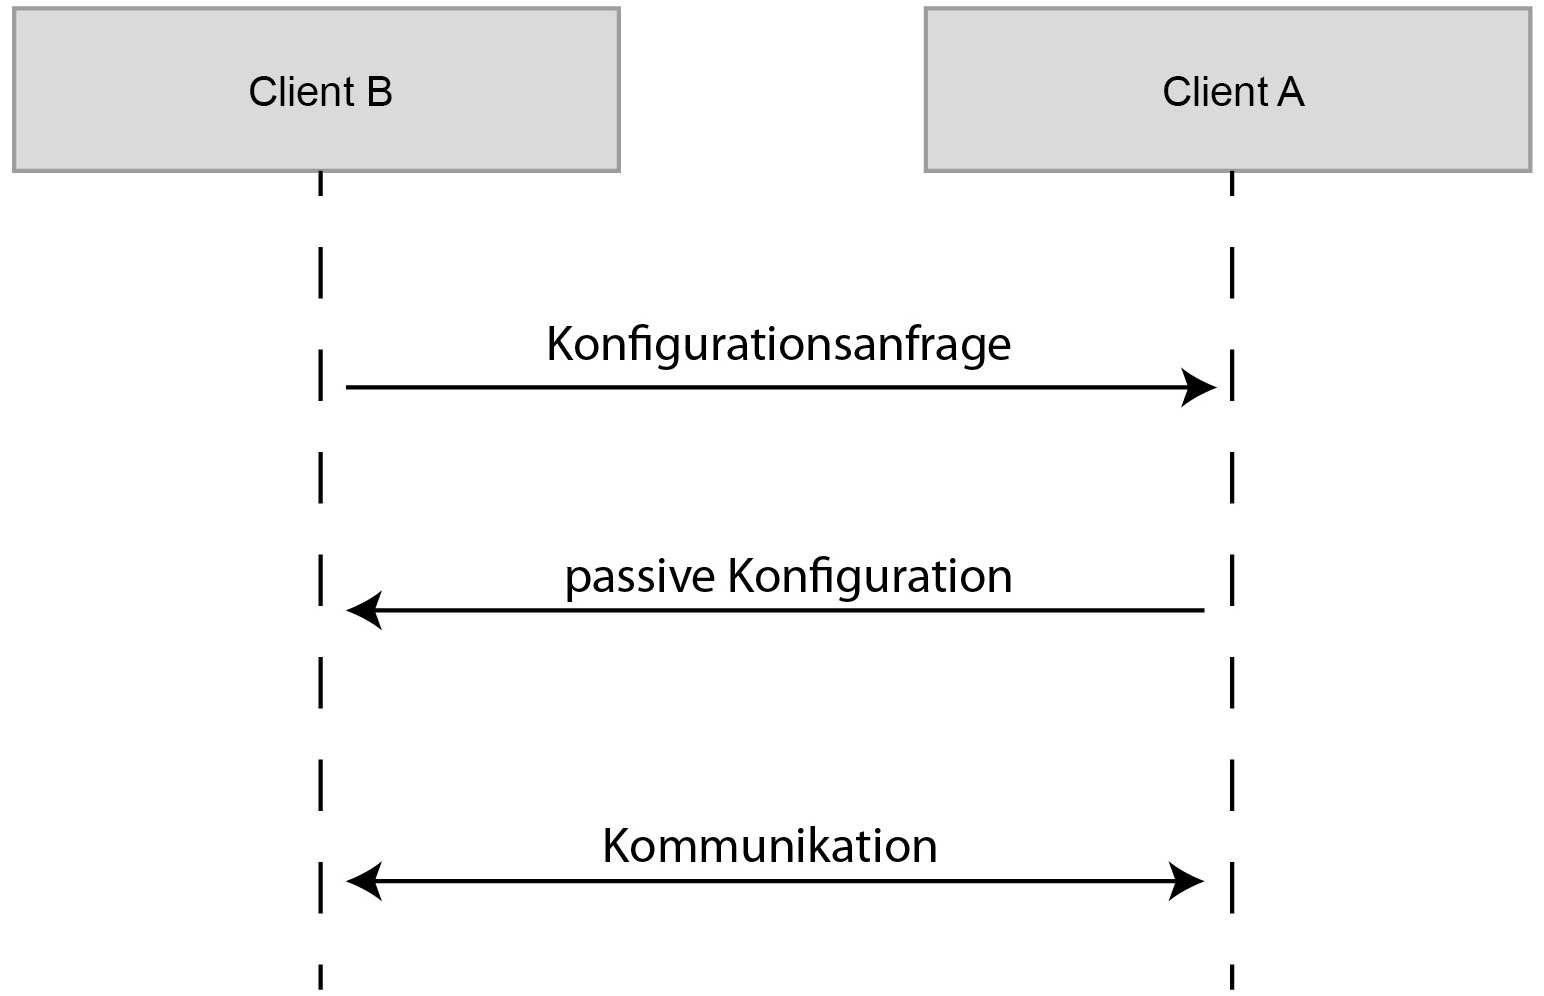
\includegraphics[width=.75\textwidth]{../img/passiveConfiguration}
\caption{Ablauf der passiven Konfiguration}
\label{lst:passiveConfiguration}
\end{figure}

\FloatBarrier
%\begin{lstlisting}[keepspaces=true,numbers=none,label=lst:passiveConfiguration,caption=Ablauf der passiven Konfiguration,xleftmargin=.2\textwidth, xrightmargin=.2\textwidth]
%Client B                            Client A
%  |                                       |
%  |         Konfigurationsanfrage         |
%  |-------------------------------------->|
%  |                                       |
%  |         passive Konfiguration         |
%  |<--------------------------------------|
%  |                                       |
%  |             Kommunikation             |
%  |<------------------------------------->|
%\end{lstlisting}